%!TEX root = ../thesis.tex

\subsection{結果}

結果だよ

\begin{figure}[tbp]
  \centering
  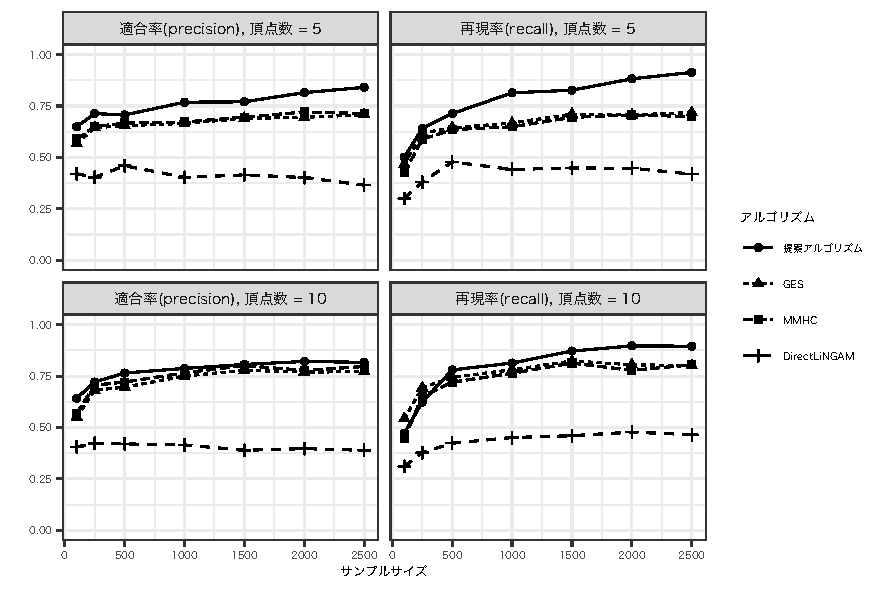
\includegraphics[width=13cm, bb=9 9 358 434]{./picture/plot_gaussian.pdf}
  \caption{連続変数の誤差変数が正規分布に従う提案モデルにおける各アルゴリズムの精度比較}
  \label{fig:plot_gaussian}
\end{figure}

\begin{figure}[tbp]
  \centering
  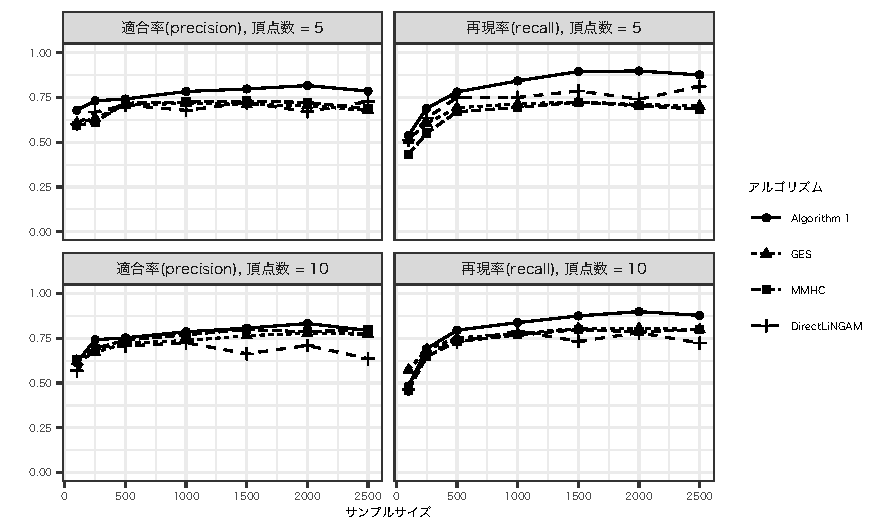
\includegraphics[width=13cm, bb=9 9 358 434]{./picture/plot_uniform.pdf}
  \caption{連続変数の誤差変数が一様分布に従う提案モデルにおける各アルゴリズムの精度比較}
  \label{fig:plot_uniform}
\end{figure}
